\subsubsection{\stid{6.02} LLNL ATDM Software Technologies}

%%%%%%%%%%%%%%%%%%%%%%%%%%%%%%%%%%%%%%%%%%%%%%%%%%%%%%%%%%%%%%%%%%%%%
\paragraph{Overview} \leavevmode \\

\textbf{Spack} is a package manager for
HPC~\cite{stewart+:sc19-spack-bof,gamblin+:sc19-spack-tutorial,gamblin+:lanl-spack-tutorial-2019,gamblin+:doe-nsf-spack-tutorial,baber+:pearc19-spack-tutorial,gamblin+:isc19-spack-tutorial,gamblin+:ecp19-spack-roundtable,gamblin+:ecp19-spack-tutorial,gamblin+:sc18-spack-bof,gamblin+:sc18-spack-tutorial,gamblin+:ecp18-spack-sotu,gamblin+:ecp18-spack-tutorial,gamblin+:sc17-spack-tutorial,gamblin:hpckp17,gamblin+:llnl-spack-tutorial-17,gamblin+:sc16-spack-tutorial}.
It automates the process of downloading, building, and installing
different versions of HPC applications, libraries, and their
dependencies.  Facilities can manage multi-user software deployments, and
developers and users can manage their own stacks separately.  Spack
enables complex applications to be assembled from components, lowers
barriers to reuse, and allows builds to be reproduced easily.

The \textbf{MFEM} library
\cite{MFEM,mfem_paper_2020} is focused on providing high-performance mathematical algorithms
and finite element discretizations to next-gen high-order ECP/ATDM
applications. A main component of these efforts is the development of
ATDM-specific physics enhancements in the finite element algorithms in
MFEM and the MFEM-based BLAST Arbitrary Lagrangian-Eulerian (ALE)
code \cite{BLAST}, in order to provide efficient discretization
components for LLNL's ATDM efforts, including the MARBL application
(ECP's LLNLApp).

A second main task in the MFEM project is the development of unique unstructured
adaptive mesh refinement (AMR) algorithms in MFEM, that focus on generality,
parallel scalability, and ease of integration in unstructured mesh
applications. The new AMR capabilities can benefit a variety of ECP apps that
use unstructured meshes, as well as many other applications in industry and the
SciDAC program.

Another aspect of the work is the preparation of the MFEM finite element library
and related codes for exascale platforms by using mathematical algorithms and
software implementations that exploit increasing on-node concurrency targeting
multiple complex architectures (e.g. GPUs). This part of the project is
synergistic with and leverages efforts from the ECP CEED co-design center.

MFEM is an open-source finite element library with ~3000 downloads/year from 70+
countries. It is freely available at \url{mfem.org}, on GitHub
at \url{github.com/mfem}, where the MFEM community includes more than 165
members), as well as via Spack and OpenHPC. The application outreach and the
integration in the ECP ecosystem is further facilitated by MFEM's participation
in ECP's xSDK project.

\textbf{RAJA}, \textbf{CHAI}, and \textbf{Umpire} are providing software libraries that enable
application and library developers to meet advanced architecture
portability challenges. The project goals are to enable writing
performance portable computational kernels and coordinate complex
heterogeneous memory resources among components in a large integrated
application. These libraries enhance developer productivity by insulating
them from much of the complexity associated with parallel programming
model usage and system-specific memory concerns.

The software products provided by this project are three complementary
and interoperable libraries:

\begin{enumerate}

\item {\bf RAJA}: Software abstractions that enable C++ developers to write
    performance portable (i.e., single-source) numerical kernels (loops).

\item {\bf CHAI}: C++ ``managed array'' abstractions that enable transparent
    and automatic copying of application data to memory spaces at run
    time as needed based on RAJA execution contexts.

\item {\bf Umpire}: A portable memory resource management library that provides
    a unified high-level API in C++, C and FORTRAN for resource
    discovery, memory provisioning, allocation, transformation, and
    introspection.

\end{enumerate}

Capabilities delivered by these software efforts are needed to manage the
diversity and uncertainty associated with current and future HPC
architecture design and software support. Moving forward, ECP
applications and libraries need to achieve performance portability:
without becoming bound to particular (potentially limiting) hardware or
software technologies, by insulating numerical algorithms from
platform-specific data and execution concerns, and without major
disruption as new machine, programming models, and vendor software become
available.

These libraries in development in this project are currently used in
production ASC applications at Lawrence Livermore National Laboratory
(LLNL) and receive most of their support from the LLNL national security
application project. They are also being used or being explored/adopted
by several ECP application and library projects, including: LLNL ATDM
application, GEOS (Subsurface), SW4 (EQSIM), MFEM (CEED co-design),
DevilRay (Alpine), and SUNDIALS.

\textbf{Flux}~\cite{Ahn:2014:Flux,FluxSC18} is a next-generation resource
management and scheduling software framework under active development at
LLNL. This ECP project significantly augments the design and development
of this framework to address two specific technical challenges pertaining
to exascale computing.

\begin{enumerate}
\item Provide Flux as a portable user-level scheduling solution for complex
      exascale workflows

\item Provide capabilities for co-scheduling, high throughput, task
      coordination, and high portability.

\item Develop a resource model capable of portably representing job
      requirements of exascale systems.

\item Provide Flux as the system resource manager and scheduler for exascale
      systems.
\end{enumerate}

Major efforts include developing and deploying additional capabilities
such as management and scheduling of a diverse set of emerging workflows
as well as a diverse set of exascale resources (e.g., power and burst
buffers). The project strives to do this through co-design efforts with
major workflow management software development teams within ASC (i.e.,
LLNL’s UQPipeline), ECP/ATDM programs, and exascale computing hardware
vendors themselves. Because Flux’s design allows it to be used as a
user-space scheduling tool, it is suitable for co-development with other
workflow systems that require advanced scheduling capabilities. As a
system tool, it is a potential replacement for resource managers such as
SLURM, providing more advanced scheduling capabilities with full
awareness of resources beyond just nodes and CPUs (e.g., filesystems,
power, accelerators).

\textbf{AID} (Advanced Infrastructure for Debugging) provides an advanced
debugging, code-correctness and testing toolset to facilitate
reproducing, diagnosing and fixing bugs within HPC applications. The
current capabilities include:

\begin{itemize}
\item STAT (highly scalable lightweight debugging tool);
\item Archer (low-overhead OpenMP data race detector);
\item ReMPI/NINJA (scalable record-and-replay and smart noise injector for MPI); and
\item FLiT/FPUChecker (floating-point correctness checking tool suite).
\end{itemize}

Major efforts include developing and deploying additional capabilities
within the team’s toolset for exascale systems and integrating them to
ASC and ECP/ATDM codes. The team strives to do this through co-design
efforts with both large HPC code teams and exascale computing hardware
vendors themselves.

\textbf{Caliper} is a program instrumentation and performance measurement
framework. It is designed as a performance analysis toolbox in a library,
allowing one to bake performance analysis capabilities directly into
applications and activate them at runtime. Caliper can be used for
lightweight always-on profiling or advanced performance engineering use
cases, such as tracing, monitoring, and auto-tuning. It is primarily
aimed at HPC applications, but works for any C/C++/Fortran program on
Unix/Linux.


%%%%%%%%%%%%%%%%%%%%%%%%%%%%%%%%%%%%%%%%%%%%%%%%%%%%%%%%%%%%%%%%%%%%%
\paragraph{Key  Challenges} \leavevmode \\

\subparagraph{Spack:}
Spack makes HPC software complexity manageable. Obtaining optimal
performance on supercomputers is a difficult task; the space of possible
ways to build software is combinatorial in size, and software reuse is
hindered by the complexity of integrating a large number of packages and
by issues such as binary compatibility.  Spack makes it easy to build
optimized, reproducible, and reusable HPC software.

\subparagraph{MFEM:}
The key challenges addressed by the LLNL ATDM Mathematical Libraries project are:

\noindent
{\bf \em Robust high-order finite element methods for ALE compressible flow.}
While high-order methods offer significant advantages in terms of HPC performance,
their application to complicated ALE problems requires careful considerations to
control oscillations and ensure accuracy.

\begin{figure}[htb]
\centering
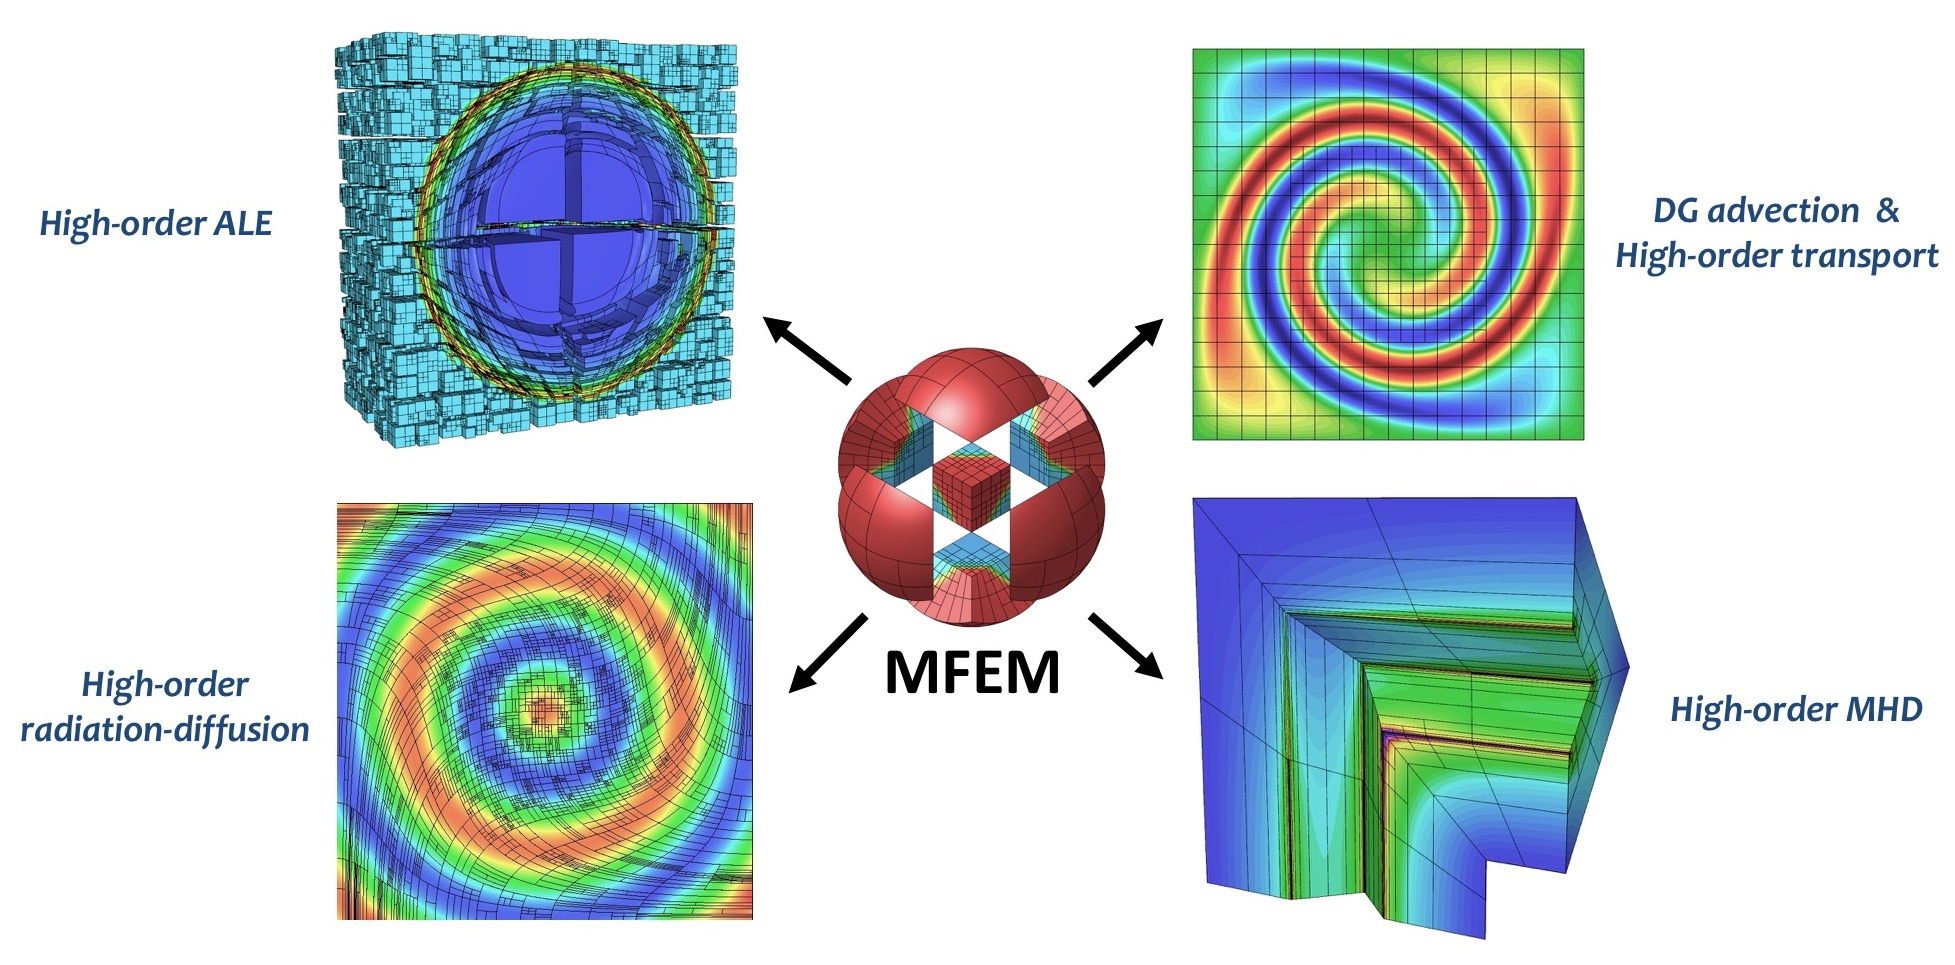
\includegraphics[width=\textwidth]{projects/2.3.6-NNSA/2.3.6.02-LLNL-ATDM/mfem-amr}
\caption{\label{fig:mfem-amr}AMR implementation in MFEM allows many applications to benefit from non-conforming adaptivity, without significant changes in their codes.}
\end{figure}

\noindent
{\bf \em Scalable algorithms for unstructured adaptive mesh refinement.}
Adaptive mesh refinement is a common way to increasing application efficiency
in problems with localized features. While block-structured AMR has been
well-studied, applying AMR in unstructured settings is challenging, especially
in terms of derefinement, anisotropic refinement, parallel rebalance and
scalability.

\noindent
{\bf \em GPU porting of finite element codes.}
Due to the relatively high complexity of the finite element machinery, MFEM,
BLAST and related codes use object-oriented C++ design that allows generality
and flexibility, but poses challenges in terms of porting to GPU architectures.
Finding the right balance between generality and performance in the GPU context
is an important challenge for many finite element-based codes that remains
outstanding in the current software and programming model environment.

\subparagraph{RAJA/Umpire/CHAI:}
Exascale machines are expected to be very diverse, with different GPU,
threading, memory models, and node architectures.  A parallelization
strategy that works well for one machine may not work well for another,
but application developers cannot afford to develop multiple versions of
their code for each machine they support.  Rather, the application must
be written using higher-level abstractions, and adapted at a lower level,
with minimal programmer effort, to specific machines.  RAJA, Umpire, and
CHAI addres this by giving applicationst the flexibility to adapt and
tune for many target machines, using the same high level kernel
formulations.  In other words they separate the concerns of performance
and correctness and avoid a combinatorial explosion of code versions for
the exascale ecosystem.

In addition to performance portability, RAJA, Umpire, and CHAI
specifically target the porting issues faced by legacy codes.  Where
other performnance portability frameworks may require a larger up-front
investment in data structures and code restructuring, RAJA, Umpire, and
CHAI are non-invasive and allow codes to adopt strategies for loop
parallelism, data layout tuning, and memory management separately.
Legacy applicaitons need not adopt all three at once; they can gradually
integrate each framework, at their own pace, with a minimal set of code
modifications.

\subparagraph{Flux:}
Exascale resource management is particularly complex as it requires us to
manage both the complexity of workloads (workflows, jobs, and services)
as well as the increasing complexity of exascale machines themselves.
Exascale systems may have diverse node types with CPUs, GPUs, burst
buffers, and other independently allocatable hardware resources. Jobs
must be mapped to these systems generically -- one application must be
able to run protably {\it and} with high performance or throughput on
{\it any} exascale machine.  Flux aims to save application developers the
pain of configuring and setting up their applciations and workflows
across multiple machine, and to enable massive ensembles and workflows to
run scalably on these machines.

\subparagraph{AID:}
Debugging parallel applications running on supercomputers is extremely
challenging.  greater challenges.  Supercomputers may contain very high
numbers of compute cores and multiple GPUs, and applications running on
such systems must rely on multiple communication and synchronization
mechanisms as well as compiler optimization options to effectively
utilize the hardware resources. These complexities often produce errors
that occur only occasionally, even when run with the exact same input on
the same hardware. These so-called non-deterministic bugs are remarkably
challenging to catch due in large part to difficulty in reproducing
them. Some errors may not even reproduce when being debugged, as the act
of debugging may perturb the execution enough to mask the bug.  To find
and fix these errors, programmers currently must devote a large amount of
effort and machine time.

\subparagraph{Caliper:}
Caliper addresses the challenges of providing {\it meaningful}
measurements for large applications.  Often, measurements of FLOPs,
timings, data movement, and other quantities are not assocciated with key
application constructs that give them meaning.  For example, we may know
the number of floating point instructions over an entire applciation run,
but if we do not know the number of mesh elements or the particular
physics phase associated with the measurement, we may be unable to
determine whether the FLOPS achieved are good or bad.  Caliper separates
these concerns: application developers can instrument the phases other
context in their code, and performance analysts and users may turn on
performance measurements that are then associated with the context.
Caliper associates meaning with HPC performance measurements.



%%%%%%%%%%%%%%%%%%%%%%%%%%%%%%%%%%%%%%%%%%%%%%%%%%%%%%%%%%%%%%%%%%%%%
\paragraph{Solution Strategy} \leavevmode \\

\subparagraph{Spack:}
Spack provides a domain-specific language for templated build recipes.
It provides a unique infrastructure called the {\it concretizer}, which
solves the complex constraint problems that arise in HPC dependency
resolution.  Developers can specify builds {\it abstractly}, and Spack
automates the tedious configuration process and drives the build. Spack
also includes online services to host recipes, code, and binaries for
broad reuse.  These repositories are maintained by Spack's very active
community of contributors.

\subparagraph{MFEM:}
The MFEM team has performed and documented a lot of research in
high-performance mathematical algorithms and finite element discretizations
of interest to ATDM applications
\cite{BLAST18,BLASTFCT18,BLASTFCT17,BLAST16,BLAST14,BLAST13,BLAST12,BLAST11}.
Our work has demonstrated that the high-order finite element approach can
successfully handle coupled multi-material ALE, radiation-diffusion and MHD.
We have also shown how high-order methods can be adapted for monotonicity
(positivity preservation), handling of artificial viscosity (shock capturing),
sub-zonal physics via closure models, etc.

To enable many applications to take advantage of unstructured mesh adaptivity,
the MFEM team is developing AMR algorithms at library level, targeting both
{\em conforming} local refinement on simplex meshes and {\em non-conforming}
refinement for quad/hex meshes. Our approach is fairly general, allowing for
any high-order finite element space, H1, H(curl), H(div), on any high-order
curved mesh in 2D and 3D, arbitrary order hanging nodes, anisotropic refinement,
derifenement and parallel load balancing.
An important feature of our library approach is that it is independent of
the physics, and thus easy to incorporate in apps, see Figure \ref{fig:mfem-amr}.

As part of the efforts in the ECP co-design Center for Efficient Exascale
Discretizations (CEED), the MFEM team is also developing mathematical algorithms
and software implementations for finite element methods that exploit increasingq
on-node concurrency targeting multiple complex architectures (e.g. GPUs). This
work includes the libCEED low-level API library, the Laghos miniapp, and several
other efforts available through CEED.

To reach its many customers and partners in NNSA, DOE Office of Science,
academia and industry, the MFEM team delivers regular releases on GitHub
(e.g., mfem-4.0 in 2019 and mfem-4.1 in 2020) that include
detailed documentation and many example codes.  Code quality is ensured
by smoke tests with Travis CI on Linux, Mac, Windows and nightly
regression testing at LLNL.

\subparagraph{RAJA/Umpire/CHAI:}
RAJA, Umpire, and CHAI leverage the abstraction mechanisms available in
modern C++ (C++11 and higher) compilers, such as Lambdas, policy
templates, and constructor/destructor (RAII) patterns for resource
management.  They aim to provide performance portability at the {\it
library} level, and they do not require special support from compilers.
Targeting this level of the software stack gives DOE developers the
flexibility to leverage standard parallel programming models like CUDA
and OpenMP, without strictly {\it depending} on robust compiler support
for these APIs.  If necessary features are unavailable in compilers,
library authors are not dependent on vendors for support, and they do not
need to wait for these programming models to be fully implemented.  These
libraries allow applications to work correctly and performantly even if
some functionality from OpenMP, CUDA, threading, etc. is missing.

\subparagraph{Flux:}
Flux implements {\it hierarchical} scheduling.  Ultimately, it will be
usable either as a full system resource manager, {\it or} as a scheduler
for a single workflow {\it within} another allocation, {\it or} as both.
Flux allows application-level workloads to choose their own scheduleing
policies and to specify concisely and portably the types of resources
they need to run on a range of machines.  Unlike prior approaches like
SLURM, which use a on-size-fits-all scheduling and job management
appoach, Flux allows the system to set global allocation policies, but
users can instnatiate their own schedulers and request specific resources
within an allocation.  With Flux, users have the control over policy and
scalability that was previously only tunable at the system level.

\subparagraph{AID:}

\begin{figure}[htb]
\centering
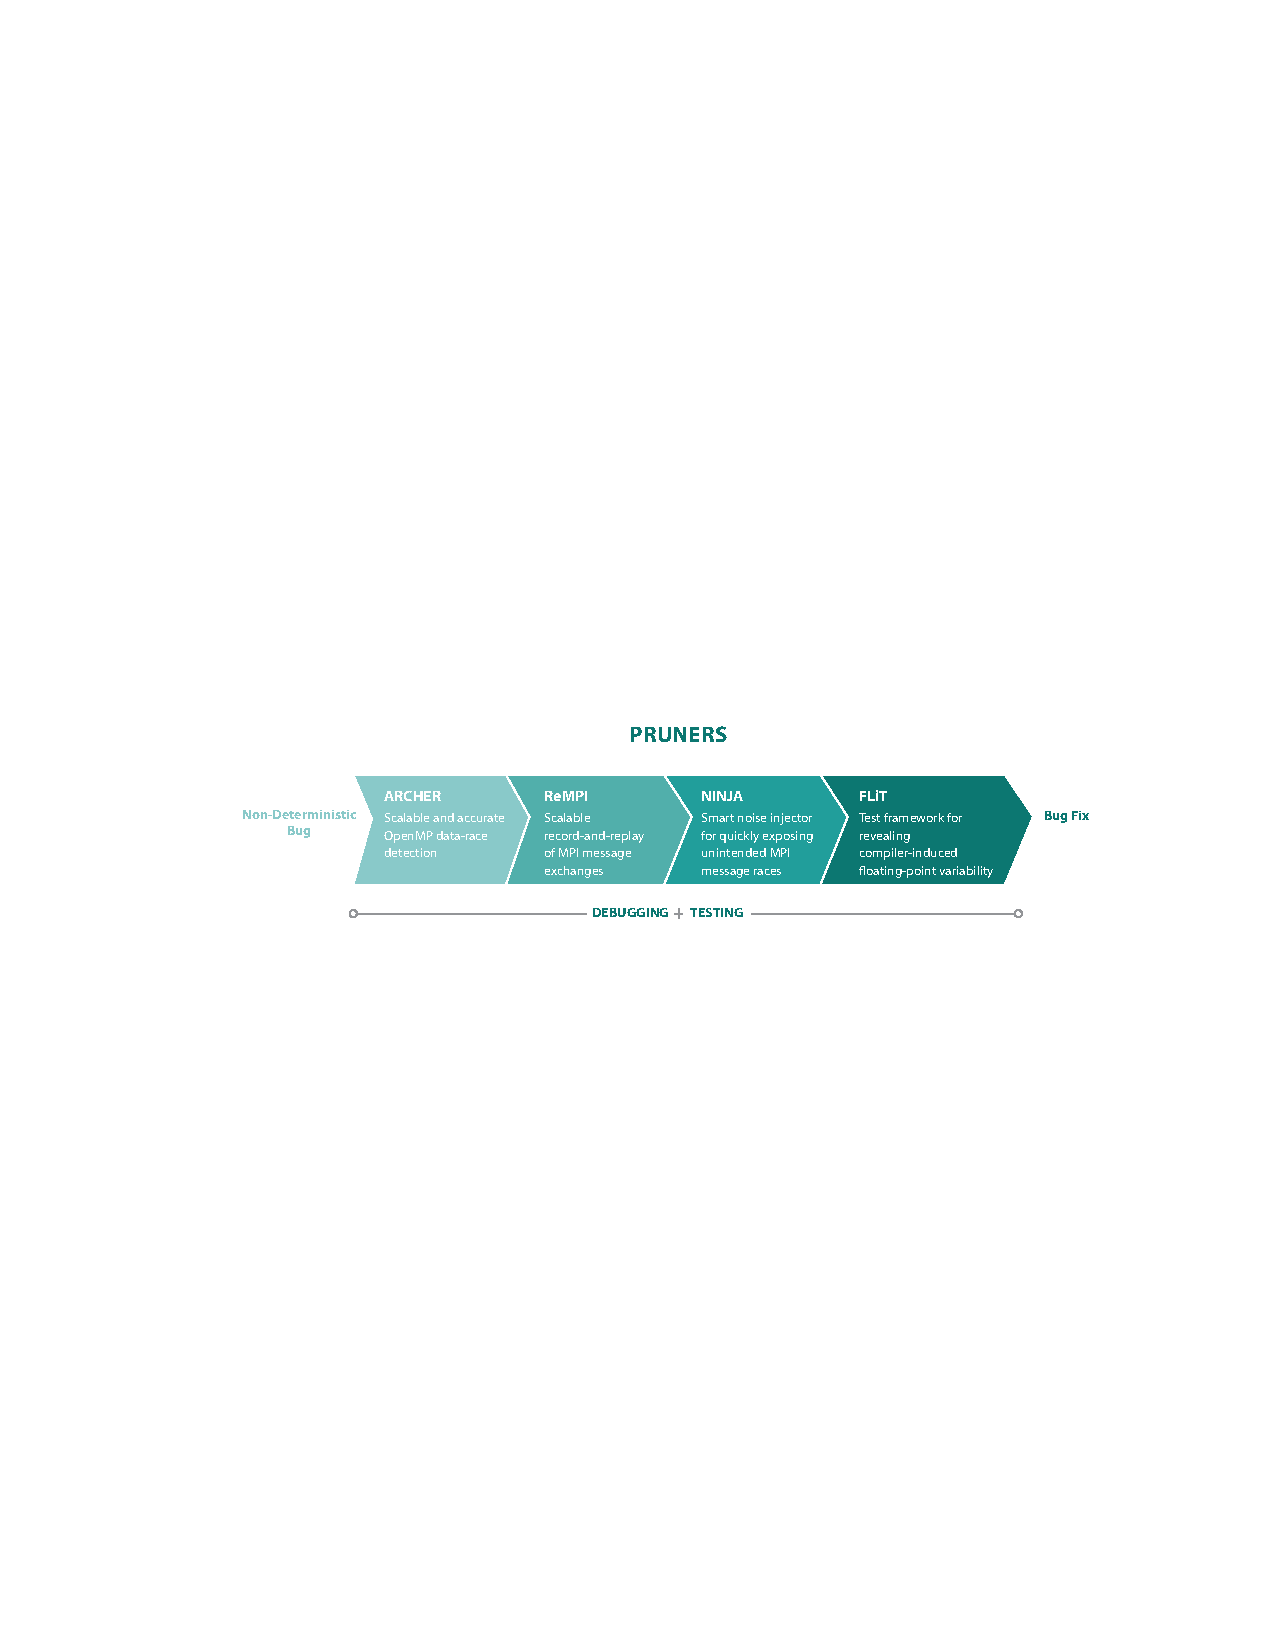
\includegraphics[width=\textwidth]{projects/2.3.6-NNSA/2.3.6.02-LLNL-ATDM/pruners}
\caption{
STAT, Archer, NINJA, and FliT: a continuum of debugging tools for exascale.
}
\end{figure}

Debugging a parallel code can be extremely difficult, and the most
exhaustive approaches for finding errors can require a large amount of
time to run.  For example, understanding all of the potential
interleavings of parallel threaded code requires combinatorial runtime
with respect to the number of threads.  It is not feasible to run this
type of analysis at all times.

Our strategy is to provide a continuum of debugging tools -- from the
lightweight tools like STAT, which require only seconds to run and gives
a high level overview of a code, to Archer, which requires lightweight
code instrumentation, to replay-based fuzzing tools like ReMPI and FLiT,
which run the code in a number of configurations to detect errors.  With
a suite of tools, we can enable developers to find the most common bugs
quickly, while still being able to detect deep, hard-to-find issues given
sufficient runtime and resources.

\subparagraph{Caliper:}
Caliper is implemented as a C++ library and is linked with applications.
Application teams integrate it with their code by adding Caliper
annotations at the application level.  Contrast this with binary analysis
and DWARF line mappings used by most performance tools, which are
obtained automatiaclly but increase tool complexity and are typically
{\it not} linked with the application for regular runs.

Applications, their libraries, physics modules, and even runtime systems
can be instrumented with Caliper and measured at the same time.  All of
these layers of the application stack provide additional context to
Caliper measuements and enable deeper analysis of the relationships
between different parts of the code.



%%%%%%%%%%%%%%%%%%%%%%%%%%%%%%%%%%%%%%%%%%%%%%%%%%%%%%%%%%%%%%%%%%%%%
\paragraph{Recent Progress} \leavevmode \\


\subparagraph{Spack:}
\begin{figure}[tb]
\centering
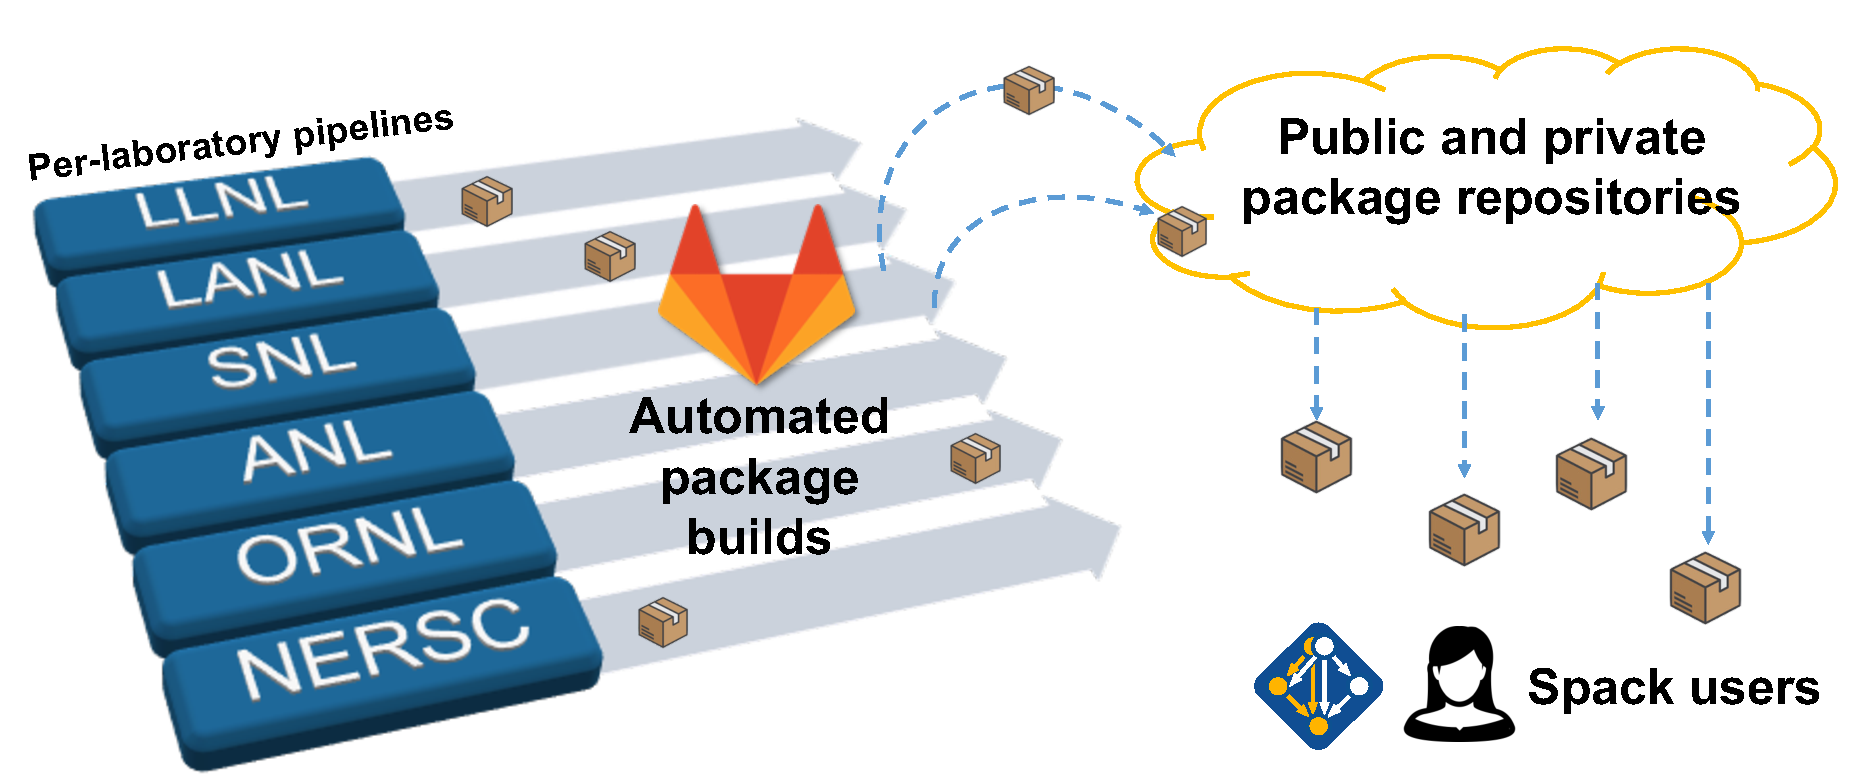
\includegraphics[width=.75\textwidth]{projects/2.3.6-NNSA/2.3.6.02-LLNL-ATDM/spack-pipelines.pdf}
\caption{Spack build pipelines at facilities will provide HPC-native binary builds for users.}
\end{figure}


\begin{itemize}
\item Produced two major software releases: Spack 0.14.0, 0.15.0, as well as multiple bug-fix releases.
\item Developed a new Spack containerize command, which can automatically generate multi-stage container build recipes from a Spack environment.
\item Completed 100\% file system lock-based parallel build capability for Spack. This capability handles both parallel build use case and on-node synchronization.
\item Worked with the tri-lab Computing Environment 2 (TCE2) team and code teams to provide Spack support and to add features for these environments. Notable achievements included hardening for Cray platforms, new features in Spack stacks, and GitLab pipeline automation for LC.
\item Deployed pull request build testing on GitHub for the first time; the entire E4S stack is now built and tested when GitHub pull requests modify parts of it.
\end{itemize}

\subparagraph{MFEM:}

\begin{figure}[tb]
\centering
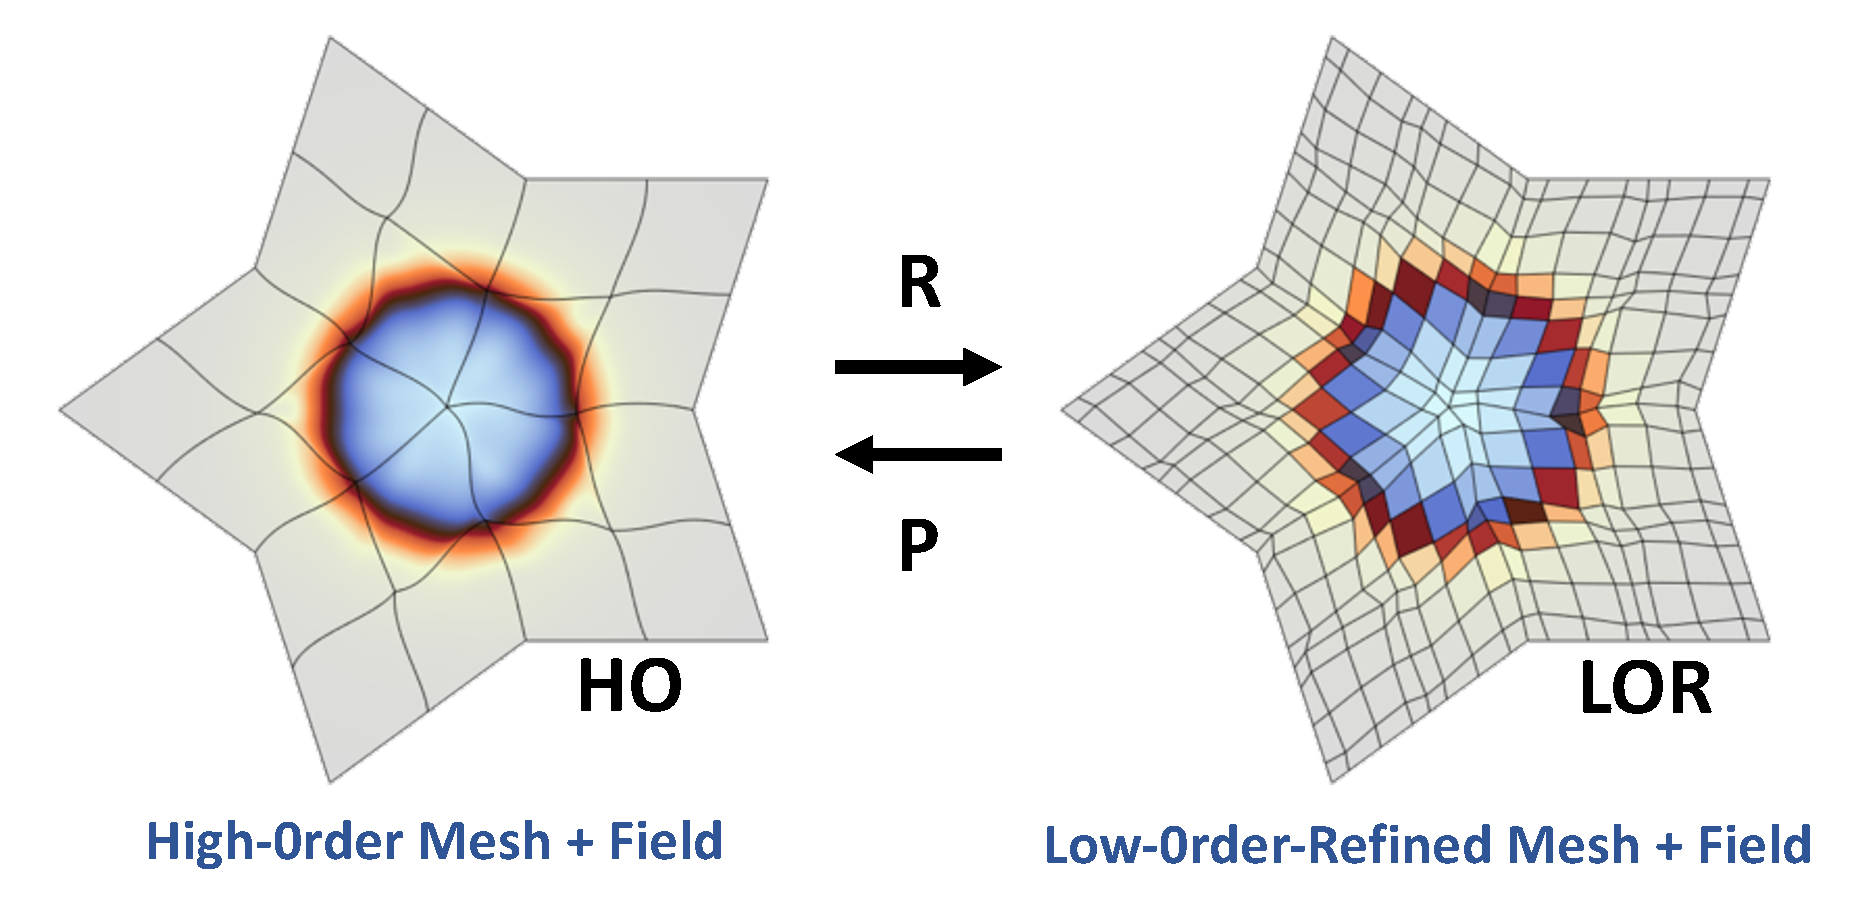
\includegraphics[width=.4\textwidth]{projects/2.3.6-NNSA/2.3.6.02-LLNL-ATDM/HO-LO}
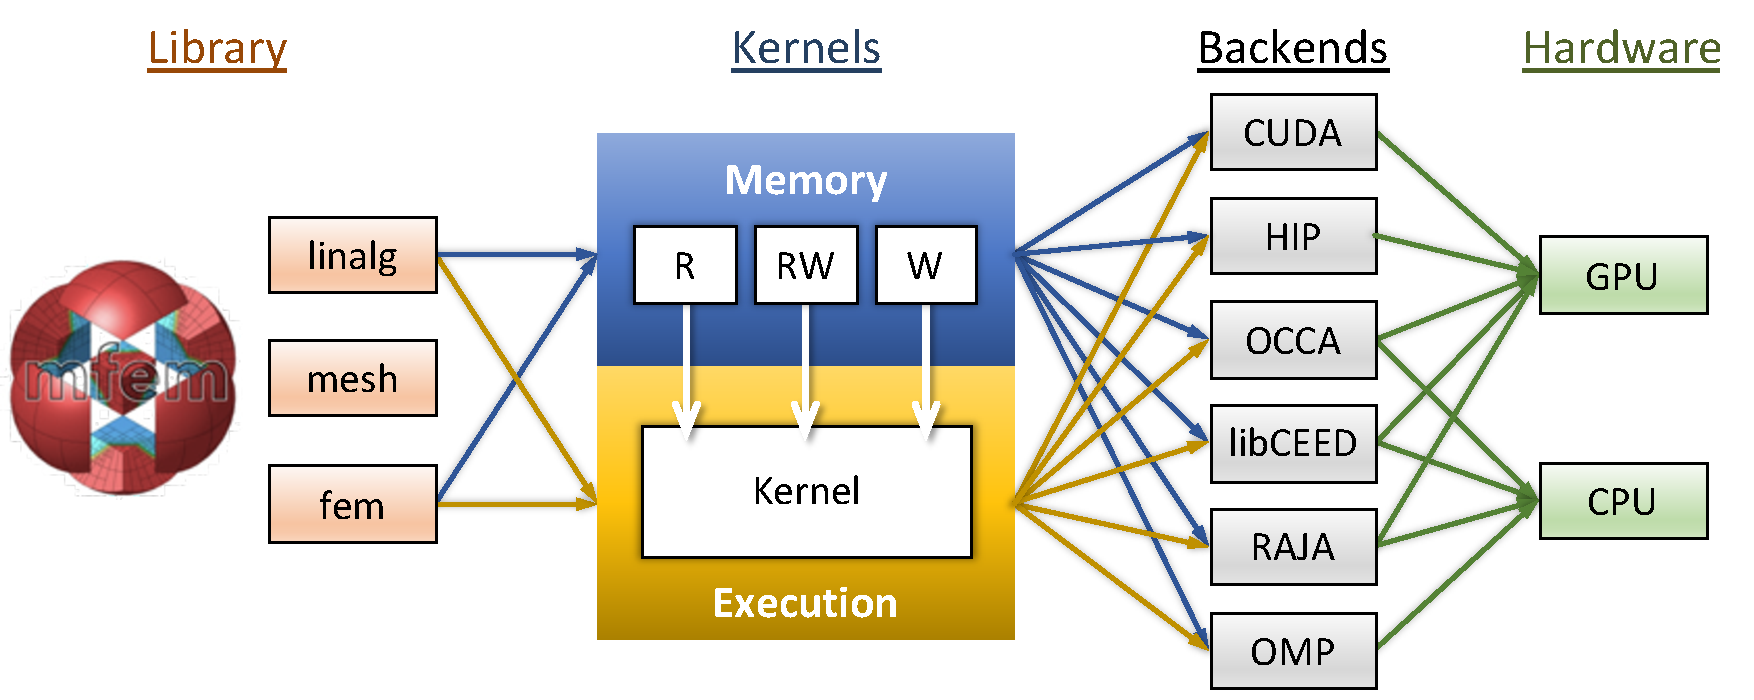
\includegraphics[width=.4\textwidth]{projects/2.3.6-NNSA/2.3.6.02-LLNL-ATDM/mfem-gpu}
\caption{The MFEM team has developed High-Order $\protect\leftrightarrow$ Low-Order Transformations and GPU support for many linear algebra and finite element operations}
\end{figure}

Selected recent highlights:
\begin{itemize}
\item Completed major software releases: Laghos-3.0, Remhos-1.0, MFEM-4.0, and MFEM-4.1. 
\item Actively engaged with GPUs and advanced partial assembly algorithms work in MARBL. Demonstrated large-scale GPU performance in ALE hydro in MFEM benchmarks, Laghos, and BLAST on Lassen. 
\item Implemented ALE discretization improvements for compressible flow in BLAST, including significant improvements in mesh optimization methods, dynamic Adaptive Mesh Refinement (AMR), and transfer between high-order and low-order-refined simulations. 

\end{itemize}

\subparagraph{RAJA/Umpire/CHAI:}
\begin{figure}[htb]
\centering
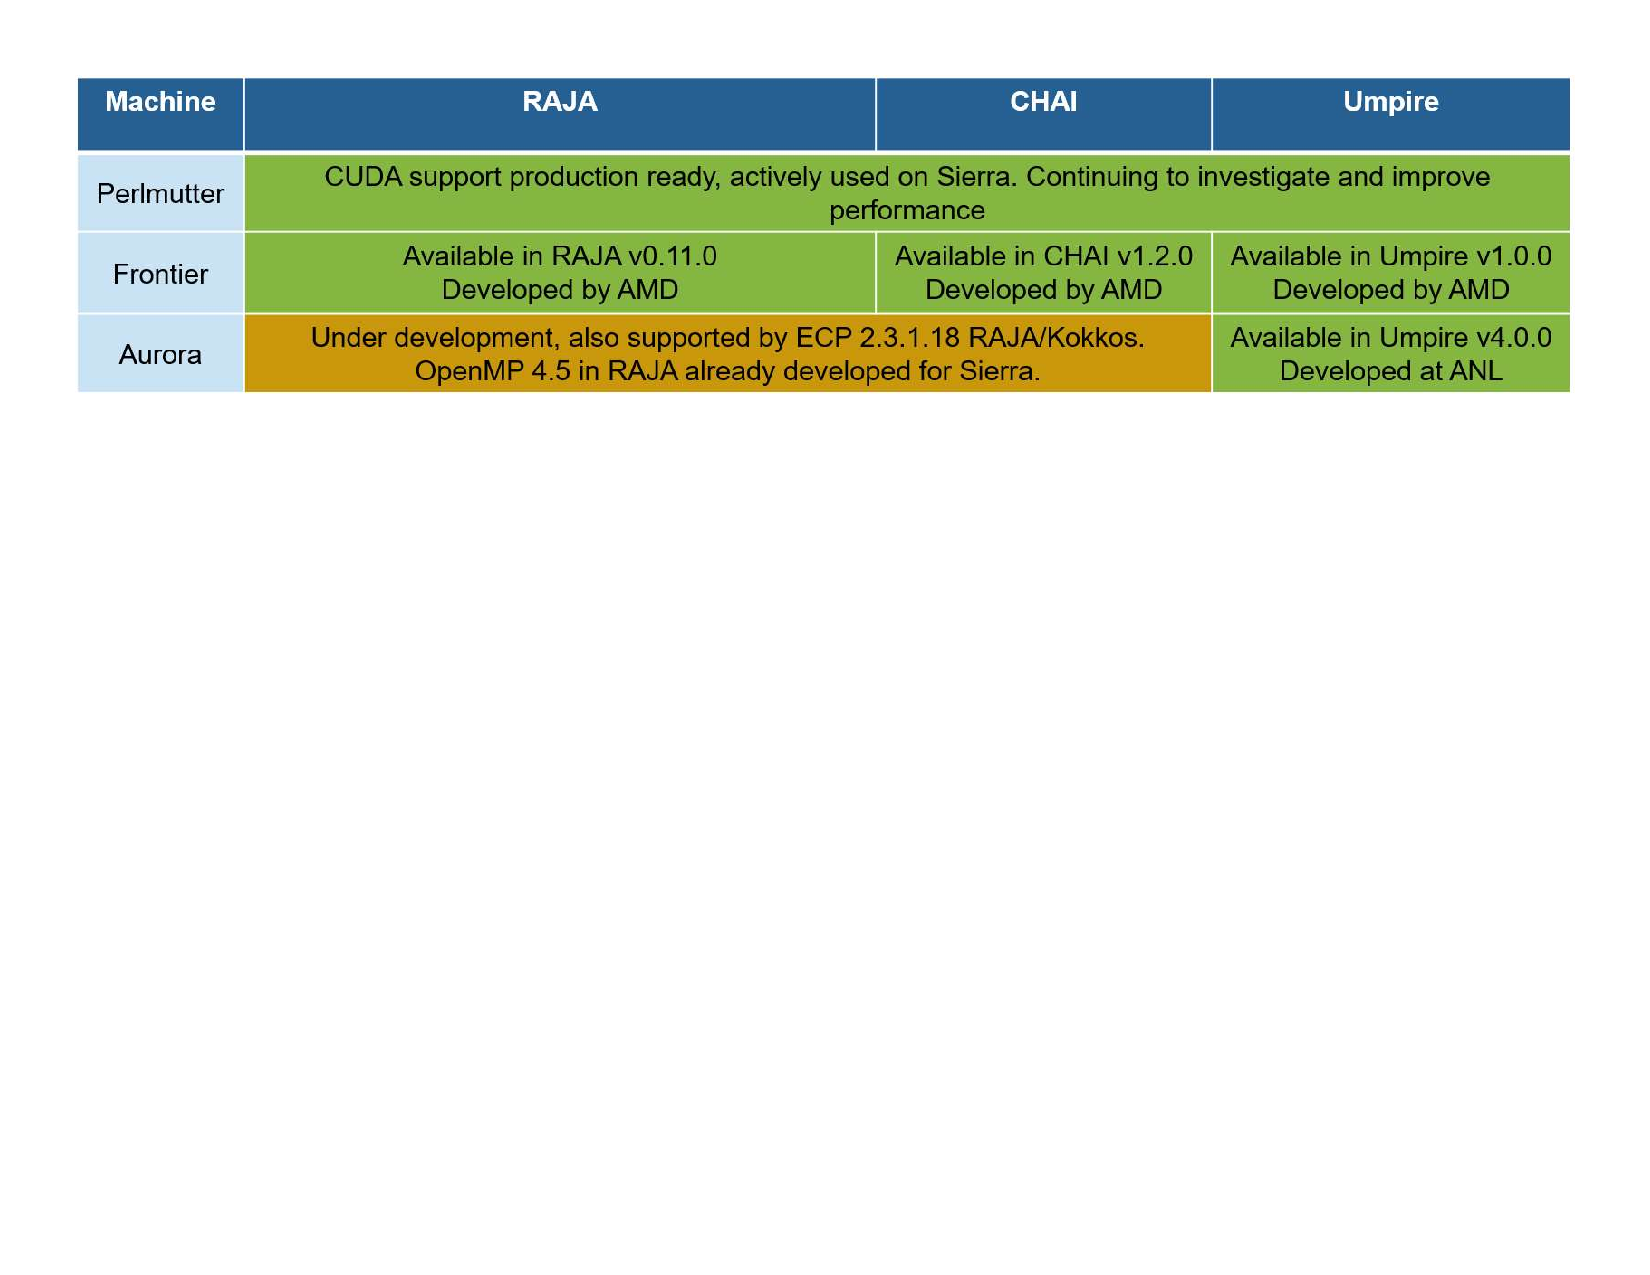
\includegraphics[width=\textwidth]{projects/2.3.6-NNSA/2.3.6.02-LLNL-ATDM/raja-umpire-chai-support}
\caption{
Status of RAJA, Umpire, and CHAI support for exascale platforms.
}
\end{figure}

\begin{itemize}
\item Developed and released support for AMD GPUs (via the HIP programming model) with RAJA, CHAI, and Umpire in preparation for El Capitan. 
\item Continued to support integration of Umpire into multiple ASC application codes.
\item Developed and delivered new capabilities to ASC applications in support of ASC milestones and user needs. 
\item Developed prototype of fully overlapped asynchronous GPU kernel execution and data transfer to optimize application performance.
\item Developed novel memory pool algorithms in Umpire to handle very large allocation counts.
\end{itemize}

\subparagraph{Flux:}
\begin{figure}[tb]
\centering
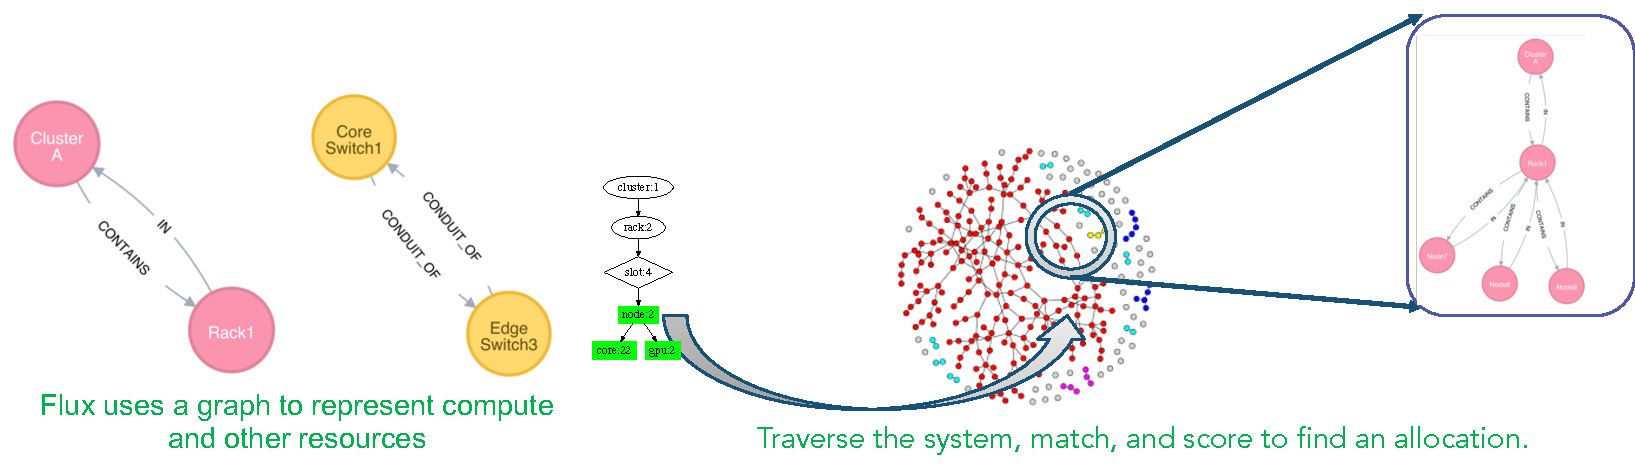
\includegraphics[width=\textwidth]{projects/2.3.6-NNSA/2.3.6.02-LLNL-ATDM/flux-resource-model.pdf}
\end{figure}

\begin{itemize}

\item Developed hierarchical scheduling tools within Flux via co-design with UQ Pipeline, demonstrating improvements across the entire lifecycle of simulation campaigns; and demonstrated that DYAD can optimize ML workflows by automatically transferring data files using Flux. 
\item Demonstrated that Fluxion, our graph-based scheduler, can uniquely enable key use cases of multitiered storage on El Capitan, driving co-design with HPE; tested AMD GPU scheduling by enabling COVID-19 workflows on Corona; demonstrated the viability of power management within Flux using Variorum, a platform-independent power library; and released MPIBIND-2. 


\end{itemize}

\subparagraph{AID:}
\begin{itemize}

\item Demonstrated that our new correctness tools (FLiT and FPChecker) can analyze large LLNL code, discovering previously unknown issues in LLNL code; and facilitated tools co-design via the El Capitan tools working group. 


\end{itemize}

\subparagraph{Caliper:}
\begin{itemize}
\item Integrated the Caliper performance analysis tools into key LLNL applications. Supported existing integration with MARBL via improvements to performance visualizations and analysis capabilities.
\end{itemize}


%%%%%%%%%%%%%%%%%%%%%%%%%%%%%%%%%%%%%%%%%%%%%%%%%%%%%%%%%%%%%%%%%%%%%
\paragraph{Next Steps} \leavevmode \\

\subparagraph{Spack:}
In FY21, the team will focus on:

\begin{itemize}
    \item Work with MARBL and other code teams to improve developer workflows support for Spack as a development tool.
    \item Improve integration testing for LLNL code teams by enabling testing for pull requests on platforms of interest to LC.
    \item Improve Spack support for GPUs, programming models, and exascale architectures.
\end{itemize}

\subparagraph{MFEM:}
\begin{itemize}
\item Develop adaptive discretizations for high-order finite element ATDM applications, including algorithms such as dynamic AMR, mesh optimization, and hp-adaptivity. 
\item Support MFEM-based ATDM applications in their transition to exascale hardware.  
\item Continue engagement with ATDM application work, develop mini-apps, and provide support.
\end{itemize}

\subparagraph{RAJA/Umpire/CHAI:}


\begin{itemize}
\item Develop and deliver new RAJA capabilities to LLNL codes to support ASC milestone and user requirements, including expanding support for overlapping kernel execution and data transfer and optimized AMD support.
\item Continue to develop and deliver Umpire capabilities to applications in support of ASC milestone and user requirements, including interprocess shared memory to support shared on-node data and expanding functionality available inside GPU kernels. 
\item Continue interactions with El Capitan Center of Excellence (COE) partners to resolve performance and correctness issues identified as application users begin testing on early access hardware. 

\end{itemize}

\subparagraph{Flux:}

\begin{itemize}
\item Demonstrate the scalable end-to-end support within Flux for: 1) smart multitiered storage scheduling and management, 2) CTI-based tool launching, 3) Variorum-enabled power monitoring/capping, 4) more versatile UQ/V\&V/ML workflow scheduling, and 5) DYAD-enabled workflow data scheduling on El Capitan early access systems. 
\end{itemize}

\subparagraph{AID:}
\begin{itemize}
\item Implement, evaluate and harden a multilevel general-purpose graphics processing unit (GPGPU) debugging/code-correctness tool suite on early applications running on Collaboration of Oak Ridge, Argonne, and Livermore (CORAL)-2 early access systems. 
\end{itemize}

\subparagraph{Caliper:}
\begin{itemize}
\item Continue SPOT and Caliper application integrations in LLNL applications. Expand tools with more GPU and MPI measurement capabilities.
\item Continue support, porting, and deployment of Caliper.
\end{itemize}
